\documentclass[12pt,notitlepage]{article}
\author{Leo Przybylski}
\usepackage{fancyhdr}
\usepackage{graphicx}
\usepackage{hyperref}
\usepackage{listings}
\usepackage[usenames,dvipsnames]{color}

\title{
\includegraphics[width=0.75\textwidth]{../../images/rsmart_base.png}\\
\includegraphics[width=0.70\textwidth]{../../images/kuali_base.png}\\rSmart
Rice Customizations and Maven}
\pagestyle{fancy}
\fancyhead{} % Clear all header fields 
\fancyhead[OL]{\sectionmark}
\fancyhead[OR]{
\includegraphics[height=26pt]{../../images/rsmart_base.png}}% 
\fancyhead[ER]{\sectionmark}
\fancyhead[EL]{
\includegraphics[height=26pt]{../../images/rsmart_base.png}}% 
\definecolor{ubergray}{RGB}{245,245,245}
\hypersetup{colorlinks}
\lstset{basicstyle=\scriptsize,
  backgroundcolor=\color{ubergray},
  breaklines=true,
  frame=single,
  includerangemarker=false}
\begin{document}
\maketitle
\tableofcontents

\abstract{When an institution wants to implement customizations and/or fixes from another rice distribution, how do these customizations get pushed out to other projects? The best way is through maven and the institution's Maven repository. The trouble is that Rice is a modular project where modules depend on the parent. It is important to keep the following in mind: \begin{itemize}
\item Original project parents
\item Do not use the org.kuali groupId
\end{itemize}
This document is about how to go about this.}

\section{Overview}

The following is the module layout for Rice:
{\ttfamily \begin{list}{|->}{\setlength{\leftmargin}{1em}}
  \item rice
    
    \begin{list}{|->}{\setlength{\leftmargin}{1em}}
    \item[\textbackslash->] client-contrib 
    \item config
      \begin{list}{|->}{\setlength{\leftmargin}{0.5em}}
      \item[\textbackslash->] access 
      \item archetype
      \item checkstyle
      \item deploy
      \item ide
      \end{list}
    \item core
      \begin{list}{|->}{\setlength{\leftmargin}{0.5em}}
      \item[\textbackslash->] api 
      \item framework
      \item impl
      \item web
      \end{list}
    \item core-service
      \begin{list}{|->}{\setlength{\leftmargin}{0.5em}}
      \item[\textbackslash->] api 
    \item framework
    \item impl
    \item web
    \end{list}
  \item db
    \begin{list}{|->}{\setlength{\leftmargin}{0.5em}}
    \item[\textbackslash->] impex
      \begin{list}{|->}{\setlength{\leftmargin}{0.5em}}
      \item[\textbackslash->] client
        \begin{list}{|->}{\setlength{\leftmargin}{0.5em}}
        \item[\textbackslash->] bootstrap
        \item demo
        \end{list}
      \item master
      \item server
        \begin{list}{|->}{\setlength{\leftmargin}{0.5em}}
        \item[\textbackslash->] bootstrap
        \item demo
        \end{list}
      \end{list}
    \item sql
    \end{list}
    
  \item development-tools
  \item dist
  \item edl
    \begin{list}{|->}{\setlength{\leftmargin}{0.5em}}
    \item[\textbackslash->] framework
      \item impl
    \end{list}
  \item impl
  \item it
    \begin{list}{|->}{\setlength{\leftmargin}{0.5em}}
    \item[\textbackslash->] config
      \item core
      \item edl
      \item impl
      \item internal-tools
      \item kcb
      \item ken
      \item kew
      \item kim
      \item krad
      \item krms
      \item ksb
      \item location
      \item vc
    \end{list}
  \item ken
    \begin{list}{|->}{\setlength{\leftmargin}{0.5em}}
    \item[\textbackslash->] api
    \end{list}
  \item kew
    \begin{list}{|->}{\setlength{\leftmargin}{0.5em}}
    \item[\textbackslash->] api
      \item framework
      \item impl
    \end{list}
  \item kim
    \begin{list}{|->}{\setlength{\leftmargin}{0.5em}}
    \item[\textbackslash->] kim-api
    \item kim-framework
    \item kim-impl
    \item kim-ldap
    \end{list} 
  \item kns
  \item krad
    \begin{list}{|->}{\setlength{\leftmargin}{0.5em}}
    \item[\textbackslash->] krad-app-framework
    \item krad-web-framework
    \end{list}
  \item krms
    \begin{list}{|->}{\setlength{\leftmargin}{0.5em}}
    \item[\textbackslash->] api
    \item framework
    \item impl
    \end{list}
  \item ksb
    \begin{list}{|->}{\setlength{\leftmargin}{0.5em}}
    \item[\textbackslash->] client-impl
    \item server-impl
    \end{list} 
  \item location
  \item sampleapp
  \item serviceregistry
  \item serviceregistry
  \item standalone
  \item web
  \end{list}
\end{list}}

Each module is a child that has a Maven parent back to the another module closer to the root parent. For example, \texttt{impl}'s parent is:
\begin{lstlisting}[numbers=left,language=xml,basicstyle=\scriptsize,backgroundcolor=\color{ubergray},caption={Impl Module Parent Definition},frame=single,breaklines=true]
<project xmlns="http://maven.apache.org/POM/4.0.0" 
     xmlns:xsi="http://www.w3.org/2001/XMLSchema-instance" 
     xsi:schemaLocation="http://maven.apache.org/POM/4.0.0 
                         http://maven.apache.org/maven-v4_0_0.xsd">
  <name>Rice Implementation</name>
  <modelVersion>4.0.0</modelVersion>
  <parent>
    <groupId>org.kuali.rice</groupId>
    <artifactId>rice</artifactId>
    <version>2.3.0-SNAPSHOT</version>
  </parent>
  <artifactId>rice-impl</artifactId>
...
...
</project>
  \end{lstlisting}

This creates a problem because if you create a new custom rice instance with a separate \emph{groupId}, it may look like this:

\begin{lstlisting}[numbers=left,language=xml,basicstyle=\scriptsize,backgroundcolor=\color{ubergray},caption={Custom Impl Module Parent Definition},frame=single,breaklines=true]
<project xmlns="http://maven.apache.org/POM/4.0.0" 
     xmlns:xsi="http://www.w3.org/2001/XMLSchema-instance" 
     xsi:schemaLocation="http://maven.apache.org/POM/4.0.0 
                         http://maven.apache.org/maven-v4_0_0.xsd">
  <name>Rice Implementation</name>
  <modelVersion>4.0.0</modelVersion>
  <parent>
    <groupId>com.rsmart.kuali.rice</groupId>
    <artifactId>rice</artifactId>
    <version>2.3.0-SNAPSHOT</version>
  </parent>
  <artifactId>rice-impl</artifactId>
...
...
</project>
  \end{lstlisting}

The problem with this is that it makes your custom impl module inherit changes from your rice parent instead of the foundation impl module. See illustration below:

\begin{figure}[hbp]
  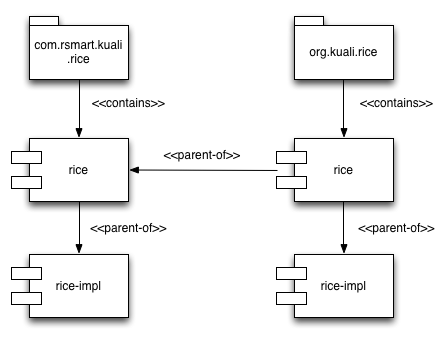
\includegraphics[width=\textwidth]{diagrams/RiceMaven1.png}
  \caption{Parallel Hierarchy from org.kuali.rice:rice as the parent}
\end{figure}

As the figure shows, this creates a parallel hierarchy where the customized \textbf{rice-impl} regards the \textbf{org.kuali.rice:rice} parent module as its parent instead of \textbf{org.kuali.rice:rice-impl} as its parent. This means whatever changes are made to the \textbf{org.kuali.rice:rice-impl} will not be reflected. 

\section{Proposal}
To summarize, we want to make it so each module is basically an overlay of the original rice module. We also want to maintain the behavior of the rice parent module.

The proposed solution involves a few parts, but by no means is it complicated. It is simply some effort because of the large number of modules in rice.
\begin{enumerate}
\item Create a project skeleton.
\item Change the module parents to point to the original rice.
\item Unpack source dependencies from \emph{org.kuali.rice} into their respective modules.
\item Make modules behave like overlays.
\end{enumerate}

\subsection*{1 Create project skeleton}
Just like overlays, we want to assume any software in our project is going on top of the original; therefore, there shouldn't be any code in it. It is basically a rice skeleton.

\subsection*{2 Change the module parents to point to original Rice modules}

Since \textbf{org.kuali.rice:rice-impl} already inherits from \textbf{org.kuali.rice:rice}, then \textbf{org.kuali.rice:rice-impl} should be made the parent instead.

\begin{figure}[hbp]
  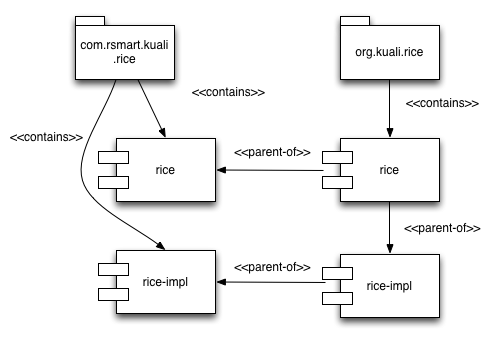
\includegraphics[width=\textwidth]{diagrams/RiceMaven2.png}
  \caption{Hierarchy with org.kuali.rice:rice-impl as the parent to com.rsmart.kuali.rice:rice-impl}
\end{figure}

\newpage 
\begin{lstlisting}[numbers=left,language=xml,basicstyle=\scriptsize,backgroundcolor=\color{ubergray},caption={Custom Impl Module Alternative Parent Definition},frame=single,breaklines=true]
<project xmlns="http://maven.apache.org/POM/4.0.0" 
     xmlns:xsi="http://www.w3.org/2001/XMLSchema-instance" 
     xsi:schemaLocation="http://maven.apache.org/POM/4.0.0 
                         http://maven.apache.org/maven-v4_0_0.xsd">
  <name>Rice Implementation</name>
  <modelVersion>4.0.0</modelVersion>
  <parent>
    <groupId>org.kuali.rice</groupId>
    <artifactId>rice-impl</artifactId>
    <version>2.3.0-SNAPSHOT</version>
  </parent>
  <artifactId>rice-impl</artifactId>
  <version>2.3.0-SNAPSHOT</version>
...
...
</project>
  \end{lstlisting}

Now the \textbf{rice-impl} module gets the benefits of being a child of the original. The \textbf{com.rsmart.kuali.rice:rice} parent should just be a dummy parent for managing the version and keeping the same version for all the other modules. The biggest issue with this proposed solution is that all the modules (there are many) would need to be updated with a new parent in order for this to work properly.

\subsection*{3 Unpack source dependencies from \emph{org.kuali.rice} into their respective modules}
We want our modules to behave like overlays. Unfortunately, overlays only exist for WAR projects and not for JAR. That is not to say we cannot create this scenario. A WAR overlay is just extracting the WAR file, throwing new source on top of it, and building a new WAR from that. We can do this with a normal JAR and the dependency plugin. 

With each snapshot and release, the Rice project publishes to the Maven repository a \emph{sources} jar for each module. This means that the \textbf{rice-impl} module has a sources jar. We can download and unpack the sources jar into an alternate location. Then, it can be compiled, and subsequently compiled into our project to build the overlay.

\begin{lstlisting}[numbers=left,language=xml,basicstyle=\scriptsize,backgroundcolor=\color{ubergray},caption={Impl Example for unpacking the org.kuali.rice:rice-impl source}]
<project xmlns="http://maven.apache.org/POM/4.0.0" 
     xmlns:xsi="http://www.w3.org/2001/XMLSchema-instance" 
     xsi:schemaLocation="http://maven.apache.org/POM/4.0.0 
                         http://maven.apache.org/maven-v4_0_0.xsd">
  <name>Rice Implementation</name>
  <modelVersion>4.0.0</modelVersion>
  <parent>
    <groupId>org.kuali.rice</groupId>
    <artifactId>rice-impl</artifactId>
    <version>2.3.0-SNAPSHOT</version>
  </parent>
  <artifactId>rice-impl</artifactId>
  <version>2.3.0-SNAPSHOT</version>
...
...
<build>
...
...
  <plugins>
...
...
    <plugin>
      <groupId>org.apache.maven.plugins</groupId>
      <artifactId>maven-dependency-plugin</artifactId>
      <version>${maven-dependency-plugin.version}</version>
      <executions>
...
...
        <execution>
          <id>unpack-rice-impl-sources</id>
          <phase>generate-sources</phase>
          <goals>
            <goal>unpack</goal>
          </goals>
          <configuration>
            <artifactItems>
              <artifactItem>
                <groupId>${project.parent.groupId}</groupId>
                <artifactId>${project.parent.artifactId}</artifactId>
                <version>${project.parent.version}</version>
                <type>jar</type>
                <classifier>sources</classifier>
                <overWrite>false</overWrite>
              </artifactItem>
            </artifactItems>
            <includes>**/*.java</includes>
            <excludes>**/*.properties,**/*.xml</excludes>
            <outputDirectory>${project.build.outputDirectory}/generated-sources/${project.parent.artifactId}</outputDirectory>
          </configuration>
        </execution>
        <execution>
          <id>unpack-rice-impl-resources</id>
          <phase>generate-resources</phase>
          <goals>
            <goal>unpack</goal>
          </goals>
          <configuration>
            <artifactItems>
              <artifactItem>
                <groupId>${project.parent.groupId}</groupId>
                <artifactId>${project.parent.artifactId}</artifactId>
                <version>${project.parent.version}</version>
                <type>jar</type>
                <classifier>sources</classifier>
                <overWrite>false</overWrite>
              </artifactItem>
            </artifactItems>
            <excludes>**/*.java</excludes>
            <includes>**/*.properties,**/*.xml</includes>
            <outputDirectory>${project.build.outputDirectory}/generated-resources/${project.parent.artifactId}</outputDirectory>
          </configuration>
        </execution>
      </executions>
    </plugin>
  </plugins>
...
...
</build>
</project>
\end{lstlisting}

The above illustrates how the dependency plugin can be used to extract the rice-impl source into a separate area for compilation at build time to produce a single jar. The above goes for all JAR projects. Rice also has a sampleapp, standalone, and web WAR project. These will simply behave like normal overlays. That means we will no need the above code. We just add the normal overlay code.

\subsection*{4 Make modules behave like overlays}
I think the above will do this for us, but I am leaving this section to outline our goal.

\section{Use Cases}

\subsection{Committing modifications to the WAR}

It should be maintained that in all cases, the preferred solution is not to modify the core code, but add new code that overrides its original behavior. Only modify core code when there is no other choice. This mostly happens with datadictionary and configuration of Spring sources. It can also happen when modifying inherent behavior that needs to process through a hierarchy or modification of private members.

\subsection{Committing modifications to a JAR}

\newpage
\listoffigures
\lstlistoflistings
\end{document}